\documentclass{report}

%%%%%%%%%%%%%%%%%%%%%%%%%%%%%%%%%
% PACKAGE IMPORTS
%%%%%%%%%%%%%%%%%%%%%%%%%%%%%%%%%


\usepackage[tmargin=2cm,rmargin=1in,lmargin=1in,margin=0.85in,bmargin=2cm,footskip=.2in]{geometry}
\usepackage{amsmath,amsfonts,amsthm,amssymb,mathtools}
\usepackage[varbb]{newpxmath}
\usepackage{xfrac}
\usepackage[makeroom]{cancel}
\usepackage{mathtools}
\usepackage{bookmark}
\usepackage{enumitem}
\usepackage{hyperref,theoremref}
\hypersetup{
	pdftitle={Assignment},
	colorlinks=true, linkcolor=doc!90,
	bookmarksnumbered=true,
	bookmarksopen=true
}
\usepackage[most,many,breakable]{tcolorbox}
\usepackage{xcolor}
\usepackage{varwidth}
\usepackage{varwidth}
\usepackage{etoolbox}
%\usepackage{authblk}
\usepackage{nameref}
\usepackage{multicol,array}
\usepackage{tikz-cd}
\usepackage[ruled,vlined,linesnumbered]{algorithm2e}
\usepackage{comment} % enables the use of multi-line comments (\ifx \fi) 
\usepackage{import}
\usepackage{xifthen}
\usepackage{pdfpages}
\usepackage{transparent}

\newcommand\mycommfont[1]{\footnotesize\ttfamily\textcolor{blue}{#1}}
\SetCommentSty{mycommfont}
\newcommand{\incfig}[1]{%
    \def\svgwidth{\columnwidth}
    \import{./figures/}{#1.pdf_tex}
}

\usepackage{tikzsymbols}
\renewcommand\qedsymbol{$\Laughey$}


%\usepackage{import}
%\usepackage{xifthen}
%\usepackage{pdfpages}
%\usepackage{transparent}


%%%%%%%%%%%%%%%%%%%%%%%%%%%%%%
% SELF MADE COLORS
%%%%%%%%%%%%%%%%%%%%%%%%%%%%%%



\definecolor{myg}{RGB}{56, 140, 70}
\definecolor{myb}{RGB}{45, 111, 177}
\definecolor{myr}{RGB}{199, 68, 64}
\definecolor{mytheorembg}{HTML}{F2F2F9}
\definecolor{mytheoremfr}{HTML}{00007B}
\definecolor{mylenmabg}{HTML}{FFFAF8}
\definecolor{mylenmafr}{HTML}{983b0f}
\definecolor{mypropbg}{HTML}{f2fbfc}
\definecolor{mypropfr}{HTML}{191971}
\definecolor{myexamplebg}{HTML}{F2FBF8}
\definecolor{myexamplefr}{HTML}{88D6D1}
\definecolor{myexampleti}{HTML}{2A7F7F}
\definecolor{mydefinitbg}{HTML}{E5E5FF}
\definecolor{mydefinitfr}{HTML}{3F3FA3}
\definecolor{notesgreen}{RGB}{0,162,0}
\definecolor{myp}{RGB}{197, 92, 212}
\definecolor{mygr}{HTML}{2C3338}
\definecolor{myred}{RGB}{127,0,0}
\definecolor{myyellow}{RGB}{169,121,69}
\definecolor{myexercisebg}{HTML}{F2FBF8}
\definecolor{myexercisefg}{HTML}{88D6D1}


%%%%%%%%%%%%%%%%%%%%%%%%%%%%
% TCOLORBOX SETUPS
%%%%%%%%%%%%%%%%%%%%%%%%%%%%

\setlength{\parindent}{1cm}
%================================
% THEOREM BOX
%================================

\tcbuselibrary{theorems,skins,hooks}
\newtcbtheorem[number within=section]{Theorem}{Theorem}
{%
	enhanced,
	breakable,
	colback = mytheorembg,
	frame hidden,
	boxrule = 0sp,
	borderline west = {2pt}{0pt}{mytheoremfr},
	sharp corners,
	detach title,
	before upper = \tcbtitle\par\smallskip,
	coltitle = mytheoremfr,
	fonttitle = \bfseries\sffamily,
	description font = \mdseries,
	separator sign none,
	segmentation style={solid, mytheoremfr},
}
{th}

\tcbuselibrary{theorems,skins,hooks}
\newtcbtheorem[number within=chapter]{theorem}{Theorem}
{%
	enhanced,
	breakable,
	colback = mytheorembg,
	frame hidden,
	boxrule = 0sp,
	borderline west = {2pt}{0pt}{mytheoremfr},
	sharp corners,
	detach title,
	before upper = \tcbtitle\par\smallskip,
	coltitle = mytheoremfr,
	fonttitle = \bfseries\sffamily,
	description font = \mdseries,
	separator sign none,
	segmentation style={solid, mytheoremfr},
}
{th}


\tcbuselibrary{theorems,skins,hooks}
\newtcolorbox{Theoremcon}
{%
	enhanced
	,breakable
	,colback = mytheorembg
	,frame hidden
	,boxrule = 0sp
	,borderline west = {2pt}{0pt}{mytheoremfr}
	,sharp corners
	,description font = \mdseries
	,separator sign none
}

%================================
% Corollery
%================================
\tcbuselibrary{theorems,skins,hooks}
\newtcbtheorem[number within=section]{Corollary}{Corollary}
{%
	enhanced
	,breakable
	,colback = myp!10
	,frame hidden
	,boxrule = 0sp
	,borderline west = {2pt}{0pt}{myp!85!black}
	,sharp corners
	,detach title
	,before upper = \tcbtitle\par\smallskip
	,coltitle = myp!85!black
	,fonttitle = \bfseries\sffamily
	,description font = \mdseries
	,separator sign none
	,segmentation style={solid, myp!85!black}
}
{th}
\tcbuselibrary{theorems,skins,hooks}
\newtcbtheorem[number within=chapter]{corollary}{Corollary}
{%
	enhanced
	,breakable
	,colback = myp!10
	,frame hidden
	,boxrule = 0sp
	,borderline west = {2pt}{0pt}{myp!85!black}
	,sharp corners
	,detach title
	,before upper = \tcbtitle\par\smallskip
	,coltitle = myp!85!black
	,fonttitle = \bfseries\sffamily
	,description font = \mdseries
	,separator sign none
	,segmentation style={solid, myp!85!black}
}
{th}


%================================
% LENMA
%================================

\tcbuselibrary{theorems,skins,hooks}
\newtcbtheorem[number within=section]{Lenma}{Lenma}
{%
	enhanced,
	breakable,
	colback = mylenmabg,
	frame hidden,
	boxrule = 0sp,
	borderline west = {2pt}{0pt}{mylenmafr},
	sharp corners,
	detach title,
	before upper = \tcbtitle\par\smallskip,
	coltitle = mylenmafr,
	fonttitle = \bfseries\sffamily,
	description font = \mdseries,
	separator sign none,
	segmentation style={solid, mylenmafr},
}
{th}

\tcbuselibrary{theorems,skins,hooks}
\newtcbtheorem[number within=chapter]{lenma}{Lenma}
{%
	enhanced,
	breakable,
	colback = mylenmabg,
	frame hidden,
	boxrule = 0sp,
	borderline west = {2pt}{0pt}{mylenmafr},
	sharp corners,
	detach title,
	before upper = \tcbtitle\par\smallskip,
	coltitle = mylenmafr,
	fonttitle = \bfseries\sffamily,
	description font = \mdseries,
	separator sign none,
	segmentation style={solid, mylenmafr},
}
{th}


%================================
% PROPOSITION
%================================

\tcbuselibrary{theorems,skins,hooks}
\newtcbtheorem[number within=section]{Prop}{Proposition}
{%
	enhanced,
	breakable,
	colback = mypropbg,
	frame hidden,
	boxrule = 0sp,
	borderline west = {2pt}{0pt}{mypropfr},
	sharp corners,
	detach title,
	before upper = \tcbtitle\par\smallskip,
	coltitle = mypropfr,
	fonttitle = \bfseries\sffamily,
	description font = \mdseries,
	separator sign none,
	segmentation style={solid, mypropfr},
}
{th}

\tcbuselibrary{theorems,skins,hooks}
\newtcbtheorem[number within=chapter]{prop}{Proposition}
{%
	enhanced,
	breakable,
	colback = mypropbg,
	frame hidden,
	boxrule = 0sp,
	borderline west = {2pt}{0pt}{mypropfr},
	sharp corners,
	detach title,
	before upper = \tcbtitle\par\smallskip,
	coltitle = mypropfr,
	fonttitle = \bfseries\sffamily,
	description font = \mdseries,
	separator sign none,
	segmentation style={solid, mypropfr},
}
{th}


%================================
% CLAIM
%================================

\tcbuselibrary{theorems,skins,hooks}
\newtcbtheorem[number within=section]{claim}{Claim}
{%
	enhanced
	,breakable
	,colback = myg!10
	,frame hidden
	,boxrule = 0sp
	,borderline west = {2pt}{0pt}{myg}
	,sharp corners
	,detach title
	,before upper = \tcbtitle\par\smallskip
	,coltitle = myg!85!black
	,fonttitle = \bfseries\sffamily
	,description font = \mdseries
	,separator sign none
	,segmentation style={solid, myg!85!black}
}
{th}



%================================
% Exercise
%================================

\tcbuselibrary{theorems,skins,hooks}
\newtcbtheorem[number within=section]{Exercise}{Exercise}
{%
	enhanced,
	breakable,
	colback = myexercisebg,
	frame hidden,
	boxrule = 0sp,
	borderline west = {2pt}{0pt}{myexercisefg},
	sharp corners,
	detach title,
	before upper = \tcbtitle\par\smallskip,
	coltitle = myexercisefg,
	fonttitle = \bfseries\sffamily,
	description font = \mdseries,
	separator sign none,
	segmentation style={solid, myexercisefg},
}
{th}

\tcbuselibrary{theorems,skins,hooks}
\newtcbtheorem[number within=chapter]{exercise}{Exercise}
{%
	enhanced,
	breakable,
	colback = myexercisebg,
	frame hidden,
	boxrule = 0sp,
	borderline west = {2pt}{0pt}{myexercisefg},
	sharp corners,
	detach title,
	before upper = \tcbtitle\par\smallskip,
	coltitle = myexercisefg,
	fonttitle = \bfseries\sffamily,
	description font = \mdseries,
	separator sign none,
	segmentation style={solid, myexercisefg},
}
{th}

%================================
% EXAMPLE BOX
%================================

\newtcbtheorem[number within=section]{Example}{Example}
{%
	colback = myexamplebg
	,breakable
	,colframe = myexamplefr
	,coltitle = myexampleti
	,boxrule = 1pt
	,sharp corners
	,detach title
	,before upper=\tcbtitle\par\smallskip
	,fonttitle = \bfseries
	,description font = \mdseries
	,separator sign none
	,description delimiters parenthesis
}
{ex}

\newtcbtheorem[number within=chapter]{example}{Example}
{%
	colback = myexamplebg
	,breakable
	,colframe = myexamplefr
	,coltitle = myexampleti
	,boxrule = 1pt
	,sharp corners
	,detach title
	,before upper=\tcbtitle\par\smallskip
	,fonttitle = \bfseries
	,description font = \mdseries
	,separator sign none
	,description delimiters parenthesis
}
{ex}

%================================
% DEFINITION BOX
%================================

\newtcbtheorem[number within=section]{Definition}{Definition}{enhanced,
	before skip=2mm,after skip=2mm, colback=red!5,colframe=red!80!black,boxrule=0.5mm,
	attach boxed title to top left={xshift=1cm,yshift*=1mm-\tcboxedtitleheight}, varwidth boxed title*=-3cm,
	boxed title style={frame code={
					\path[fill=tcbcolback]
					([yshift=-1mm,xshift=-1mm]frame.north west)
					arc[start angle=0,end angle=180,radius=1mm]
					([yshift=-1mm,xshift=1mm]frame.north east)
					arc[start angle=180,end angle=0,radius=1mm];
					\path[left color=tcbcolback!60!black,right color=tcbcolback!60!black,
						middle color=tcbcolback!80!black]
					([xshift=-2mm]frame.north west) -- ([xshift=2mm]frame.north east)
					[rounded corners=1mm]-- ([xshift=1mm,yshift=-1mm]frame.north east)
					-- (frame.south east) -- (frame.south west)
					-- ([xshift=-1mm,yshift=-1mm]frame.north west)
					[sharp corners]-- cycle;
				},interior engine=empty,
		},
	fonttitle=\bfseries,
	title={#2},#1}{def}
\newtcbtheorem[number within=chapter]{definition}{Definition}{enhanced,
	before skip=2mm,after skip=2mm, colback=red!5,colframe=red!80!black,boxrule=0.5mm,
	attach boxed title to top left={xshift=1cm,yshift*=1mm-\tcboxedtitleheight}, varwidth boxed title*=-3cm,
	boxed title style={frame code={
					\path[fill=tcbcolback]
					([yshift=-1mm,xshift=-1mm]frame.north west)
					arc[start angle=0,end angle=180,radius=1mm]
					([yshift=-1mm,xshift=1mm]frame.north east)
					arc[start angle=180,end angle=0,radius=1mm];
					\path[left color=tcbcolback!60!black,right color=tcbcolback!60!black,
						middle color=tcbcolback!80!black]
					([xshift=-2mm]frame.north west) -- ([xshift=2mm]frame.north east)
					[rounded corners=1mm]-- ([xshift=1mm,yshift=-1mm]frame.north east)
					-- (frame.south east) -- (frame.south west)
					-- ([xshift=-1mm,yshift=-1mm]frame.north west)
					[sharp corners]-- cycle;
				},interior engine=empty,
		},
	fonttitle=\bfseries,
	title={#2},#1}{def}



%================================
% Solution BOX
%================================

\makeatletter
\newtcbtheorem{question}{Question}{enhanced,
	breakable,
	colback=white,
	colframe=myb!80!black,
	attach boxed title to top left={yshift*=-\tcboxedtitleheight},
	fonttitle=\bfseries,
	title={#2},
	boxed title size=title,
	boxed title style={%
			sharp corners,
			rounded corners=northwest,
			colback=tcbcolframe,
			boxrule=0pt,
		},
	underlay boxed title={%
			\path[fill=tcbcolframe] (title.south west)--(title.south east)
			to[out=0, in=180] ([xshift=5mm]title.east)--
			(title.center-|frame.east)
			[rounded corners=\kvtcb@arc] |-
			(frame.north) -| cycle;
		},
	#1
}{def}
\makeatother

%================================
% SOLUTION BOX
%================================

\makeatletter
\newtcolorbox{solution}{enhanced,
	breakable,
	colback=white,
	colframe=myg!80!black,
	attach boxed title to top left={yshift*=-\tcboxedtitleheight},
	title=Solution,
	boxed title size=title,
	boxed title style={%
			sharp corners,
			rounded corners=northwest,
			colback=tcbcolframe,
			boxrule=0pt,
		},
	underlay boxed title={%
			\path[fill=tcbcolframe] (title.south west)--(title.south east)
			to[out=0, in=180] ([xshift=5mm]title.east)--
			(title.center-|frame.east)
			[rounded corners=\kvtcb@arc] |-
			(frame.north) -| cycle;
		},
}
\makeatother

%================================
% Question BOX
%================================

\makeatletter
\newtcbtheorem{qstion}{Question}{enhanced,
	breakable,
	colback=white,
	colframe=mygr,
	attach boxed title to top left={yshift*=-\tcboxedtitleheight},
	fonttitle=\bfseries,
	title={#2},
	boxed title size=title,
	boxed title style={%
			sharp corners,
			rounded corners=northwest,
			colback=tcbcolframe,
			boxrule=0pt,
		},
	underlay boxed title={%
			\path[fill=tcbcolframe] (title.south west)--(title.south east)
			to[out=0, in=180] ([xshift=5mm]title.east)--
			(title.center-|frame.east)
			[rounded corners=\kvtcb@arc] |-
			(frame.north) -| cycle;
		},
	#1
}{def}
\makeatother

\newtcbtheorem[number within=chapter]{wconc}{Wrong Concept}{
	breakable,
	enhanced,
	colback=white,
	colframe=myr,
	arc=0pt,
	outer arc=0pt,
	fonttitle=\bfseries\sffamily\large,
	colbacktitle=myr,
	attach boxed title to top left={},
	boxed title style={
			enhanced,
			skin=enhancedfirst jigsaw,
			arc=3pt,
			bottom=0pt,
			interior style={fill=myr}
		},
	#1
}{def}



%================================
% NOTE BOX
%================================

\usetikzlibrary{arrows,calc,shadows.blur}
\tcbuselibrary{skins}
\newtcolorbox{note}[1][]{%
	enhanced jigsaw,
	colback=gray!20!white,%
	colframe=gray!80!black,
	size=small,
	boxrule=1pt,
	title=\textbf{Note:-},
	halign title=flush center,
	coltitle=black,
	breakable,
	drop shadow=black!50!white,
	attach boxed title to top left={xshift=1cm,yshift=-\tcboxedtitleheight/2,yshifttext=-\tcboxedtitleheight/2},
	minipage boxed title=1.5cm,
	boxed title style={%
			colback=white,
			size=fbox,
			boxrule=1pt,
			boxsep=2pt,
			underlay={%
					\coordinate (dotA) at ($(interior.west) + (-0.5pt,0)$);
					\coordinate (dotB) at ($(interior.east) + (0.5pt,0)$);
					\begin{scope}
						\clip (interior.north west) rectangle ([xshift=3ex]interior.east);
						\filldraw [white, blur shadow={shadow opacity=60, shadow yshift=-.75ex}, rounded corners=2pt] (interior.north west) rectangle (interior.south east);
					\end{scope}
					\begin{scope}[gray!80!black]
						\fill (dotA) circle (2pt);
						\fill (dotB) circle (2pt);
					\end{scope}
				},
		},
	#1,
}

%%%%%%%%%%%%%%%%%%%%%%%%%%%%%%
% SELF MADE COMMANDS
%%%%%%%%%%%%%%%%%%%%%%%%%%%%%%


\newcommand{\thm}[2]{\begin{Theorem}{#1}{}#2\end{Theorem}}
\newcommand{\cor}[2]{\begin{Corollary}{#1}{}#2\end{Corollary}}
\newcommand{\mlenma}[2]{\begin{Lenma}{#1}{}#2\end{Lenma}}
\newcommand{\mprop}[2]{\begin{Prop}{#1}{}#2\end{Prop}}
\newcommand{\clm}[3]{\begin{claim}{#1}{#2}#3\end{claim}}
\newcommand{\wc}[2]{\begin{wconc}{#1}{}\setlength{\parindent}{1cm}#2\end{wconc}}
\newcommand{\thmcon}[1]{\begin{Theoremcon}{#1}\end{Theoremcon}}
\newcommand{\ex}[2]{\begin{Example}{#1}{}#2\end{Example}}
\newcommand{\dfn}[2]{\begin{Definition}[colbacktitle=red!75!black]{#1}{}#2\end{Definition}}
\newcommand{\dfnc}[2]{\begin{definition}[colbacktitle=red!75!black]{#1}{}#2\end{definition}}
\newcommand{\qs}[2]{\begin{question}{#1}{}#2\end{question}}
\newcommand{\pf}[2]{\begin{myproof}[#1]#2\end{myproof}}
\newcommand{\nt}[1]{\begin{note}#1\end{note}}

\newcommand*\circled[1]{\tikz[baseline=(char.base)]{
		\node[shape=circle,draw,inner sep=1pt] (char) {#1};}}
\newcommand\getcurrentref[1]{%
	\ifnumequal{\value{#1}}{0}
	{??}
	{\the\value{#1}}%
}
\newcommand{\getCurrentSectionNumber}{\getcurrentref{section}}
\newenvironment{myproof}[1][\proofname]{%
	\proof[\bfseries #1: ]%
}{\endproof}

\newcommand{\mclm}[2]{\begin{myclaim}[#1]#2\end{myclaim}}
\newenvironment{myclaim}[1][\claimname]{\proof[\bfseries #1: ]}{}

\newcounter{mylabelcounter}

\makeatletter
\newcommand{\setword}[2]{%
	\phantomsection
	#1\def\@currentlabel{\unexpanded{#1}}\label{#2}%
}
\makeatother




\tikzset{
	symbol/.style={
			draw=none,
			every to/.append style={
					edge node={node [sloped, allow upside down, auto=false]{$#1$}}}
		}
}


% deliminators
\DeclarePairedDelimiter{\abs}{\lvert}{\rvert}
\DeclarePairedDelimiter{\norm}{\lVert}{\rVert}

\DeclarePairedDelimiter{\ceil}{\lceil}{\rceil}
\DeclarePairedDelimiter{\floor}{\lfloor}{\rfloor}
\DeclarePairedDelimiter{\round}{\lfloor}{\rceil}

\newsavebox\diffdbox
\newcommand{\slantedromand}{{\mathpalette\makesl{d}}}
\newcommand{\makesl}[2]{%
\begingroup
\sbox{\diffdbox}{$\mathsurround=0pt#1\mathrm{#2}$}%
\pdfsave
\pdfsetmatrix{1 0 0.2 1}%
\rlap{\usebox{\diffdbox}}%
\pdfrestore
\hskip\wd\diffdbox
\endgroup
}
\newcommand{\dd}[1][]{\ensuremath{\mathop{}\!\ifstrempty{#1}{%
\slantedromand\@ifnextchar^{\hspace{0.2ex}}{\hspace{0.1ex}}}%
{\slantedromand\hspace{0.2ex}^{#1}}}}
\ProvideDocumentCommand\dv{o m g}{%
  \ensuremath{%
    \IfValueTF{#3}{%
      \IfNoValueTF{#1}{%
        \frac{\dd #2}{\dd #3}%
      }{%
        \frac{\dd^{#1} #2}{\dd #3^{#1}}%
      }%
    }{%
      \IfNoValueTF{#1}{%
        \frac{\dd}{\dd #2}%
      }{%
        \frac{\dd^{#1}}{\dd #2^{#1}}%
      }%
    }%
  }%
}
\providecommand*{\pdv}[3][]{\frac{\partial^{#1}#2}{\partial#3^{#1}}}
%  - others
\DeclareMathOperator{\Lap}{\mathcal{L}}
\DeclareMathOperator{\Var}{Var} % varience
\DeclareMathOperator{\Cov}{Cov} % covarience
\DeclareMathOperator{\E}{E} % expected

% Since the amsthm package isn't loaded

% I prefer the slanted \leq
\let\oldleq\leq % save them in case they're every wanted
\let\oldgeq\geq
\renewcommand{\leq}{\leqslant}
\renewcommand{\geq}{\geqslant}

% % redefine matrix env to allow for alignment, use r as default
% \renewcommand*\env@matrix[1][r]{\hskip -\arraycolsep
%     \let\@ifnextchar\new@ifnextchar
%     \array{*\c@MaxMatrixCols #1}}


%\usepackage{framed}
%\usepackage{titletoc}
%\usepackage{etoolbox}
%\usepackage{lmodern}


%\patchcmd{\tableofcontents}{\contentsname}{\sffamily\contentsname}{}{}

%\renewenvironment{leftbar}
%{\def\FrameCommand{\hspace{6em}%
%		{\color{myyellow}\vrule width 2pt depth 6pt}\hspace{1em}}%
%	\MakeFramed{\parshape 1 0cm \dimexpr\textwidth-6em\relax\FrameRestore}\vskip2pt%
%}
%{\endMakeFramed}

%\titlecontents{chapter}
%[0em]{\vspace*{2\baselineskip}}
%{\parbox{4.5em}{%
%		\hfill\Huge\sffamily\bfseries\color{myred}\thecontentspage}%
%	\vspace*{-2.3\baselineskip}\leftbar\textsc{\small\chaptername~\thecontentslabel}\\\sffamily}
%{}{\endleftbar}
%\titlecontents{section}
%[8.4em]
%{\sffamily\contentslabel{3em}}{}{}
%{\hspace{0.5em}\nobreak\itshape\color{myred}\contentspage}
%\titlecontents{subsection}
%[8.4em]
%{\sffamily\contentslabel{3em}}{}{}  
%{\hspace{0.5em}\nobreak\itshape\color{myred}\contentspage}



%%%%%%%%%%%%%%%%%%%%%%%%%%%%%%%%%%%%%%%%%%%
% TABLE OF CONTENTS
%%%%%%%%%%%%%%%%%%%%%%%%%%%%%%%%%%%%%%%%%%%

\usepackage{tikz}
\definecolor{doc}{RGB}{0,60,110}
\usepackage{titletoc}
\contentsmargin{0cm}
\titlecontents{chapter}[3.7pc]
{\addvspace{30pt}%
	\begin{tikzpicture}[remember picture, overlay]%
		\draw[fill=doc!60,draw=doc!60] (-7,-.1) rectangle (-0.9,.5);%
		\pgftext[left,x=-3.5cm,y=0.2cm]{\color{white}\Large\sc\bfseries Chapter\ \thecontentslabel};%
	\end{tikzpicture}\color{doc!60}\large\sc\bfseries}%
{}
{}
{\;\titlerule\;\large\sc\bfseries Page \thecontentspage
	\begin{tikzpicture}[remember picture, overlay]
		\draw[fill=doc!60,draw=doc!60] (2pt,0) rectangle (4,0.1pt);
	\end{tikzpicture}}%
\titlecontents{section}[3.7pc]
{\addvspace{2pt}}
{\contentslabel[\thecontentslabel]{2pc}}
{}
{\hfill\small \thecontentspage}
[]
\titlecontents*{subsection}[3.7pc]
{\addvspace{-1pt}\small}
{}
{}
{\ --- \small\thecontentspage}
[ \textbullet\ ][]

\makeatletter
\renewcommand{\tableofcontents}{%
	\chapter*{%
	  \vspace*{-20\p@}%
	  \begin{tikzpicture}[remember picture, overlay]%
		  \pgftext[right,x=15cm,y=0.2cm]{\color{doc!60}\Huge\sc\bfseries \contentsname};%
		  \draw[fill=doc!60,draw=doc!60] (13,-.75) rectangle (20,1);%
		  \clip (13,-.75) rectangle (20,1);
		  \pgftext[right,x=15cm,y=0.2cm]{\color{white}\Huge\sc\bfseries \contentsname};%
	  \end{tikzpicture}}%
	\@starttoc{toc}}
\makeatother


%From M275 "Topology" at SJSU
\newcommand{\id}{\mathrm{id}}
\newcommand{\taking}[1]{\xrightarrow{#1}}
\newcommand{\inv}{^{-1}}

%From M170 "Introduction to Graph Theory" at SJSU
\DeclareMathOperator{\diam}{diam}
\DeclareMathOperator{\ord}{ord}
\newcommand{\defeq}{\overset{\mathrm{def}}{=}}

%From the USAMO .tex files
\newcommand{\ts}{\textsuperscript}
\newcommand{\dg}{^\circ}
\newcommand{\ii}{\item}

% % From Math 55 and Math 145 at Harvard
% \newenvironment{subproof}[1][Proof]{%
% \begin{proof}[#1] \renewcommand{\qedsymbol}{$\blacksquare$}}%
% {\end{proof}}

\newcommand{\liff}{\leftrightarrow}
\newcommand{\lthen}{\rightarrow}
\newcommand{\opname}{\operatorname}
\newcommand{\surjto}{\twoheadrightarrow}
\newcommand{\injto}{\hookrightarrow}
\newcommand{\On}{\mathrm{On}} % ordinals
\DeclareMathOperator{\img}{im} % Image
\DeclareMathOperator{\Img}{Im} % Image
\DeclareMathOperator{\coker}{coker} % Cokernel
\DeclareMathOperator{\Coker}{Coker} % Cokernel
\DeclareMathOperator{\Ker}{Ker} % Kernel
\DeclareMathOperator{\rank}{rank}
\DeclareMathOperator{\Spec}{Spec} % spectrum
\DeclareMathOperator{\Tr}{Tr} % trace
\DeclareMathOperator{\pr}{pr} % projection
\DeclareMathOperator{\ext}{ext} % extension
\DeclareMathOperator{\pred}{pred} % predecessor
\DeclareMathOperator{\dom}{dom} % domain
\DeclareMathOperator{\ran}{ran} % range
\DeclareMathOperator{\Hom}{Hom} % homomorphism
\DeclareMathOperator{\Mor}{Mor} % morphisms
\DeclareMathOperator{\End}{End} % endomorphism

\newcommand{\eps}{\epsilon}
\newcommand{\veps}{\varepsilon}
\newcommand{\ol}{\overline}
\newcommand{\ul}{\underline}
\newcommand{\wt}{\widetilde}
\newcommand{\wh}{\widehat}
\newcommand{\vocab}[1]{\textbf{\color{blue} #1}}
\providecommand{\half}{\frac{1}{2}}
\newcommand{\dang}{\measuredangle} %% Directed angle
\newcommand{\ray}[1]{\overrightarrow{#1}}
\newcommand{\seg}[1]{\overline{#1}}
\newcommand{\arc}[1]{\wideparen{#1}}
\DeclareMathOperator{\cis}{cis}
\DeclareMathOperator*{\lcm}{lcm}
\DeclareMathOperator*{\argmin}{arg min}
\DeclareMathOperator*{\argmax}{arg max}
\newcommand{\cycsum}{\sum_{\mathrm{cyc}}}
\newcommand{\symsum}{\sum_{\mathrm{sym}}}
\newcommand{\cycprod}{\prod_{\mathrm{cyc}}}
\newcommand{\symprod}{\prod_{\mathrm{sym}}}
\newcommand{\Qed}{\begin{flushright}\qed\end{flushright}}
\newcommand{\parinn}{\setlength{\parindent}{1cm}}
\newcommand{\parinf}{\setlength{\parindent}{0cm}}
% \newcommand{\norm}{\|\cdot\|}
\newcommand{\inorm}{\norm_{\infty}}
\newcommand{\opensets}{\{V_{\alpha}\}_{\alpha\in I}}
\newcommand{\oset}{V_{\alpha}}
\newcommand{\opset}[1]{V_{\alpha_{#1}}}
\newcommand{\lub}{\text{lub}}
\newcommand{\del}[2]{\frac{\partial #1}{\partial #2}}
\newcommand{\Del}[3]{\frac{\partial^{#1} #2}{\partial^{#1} #3}}
\newcommand{\deld}[2]{\dfrac{\partial #1}{\partial #2}}
\newcommand{\Deld}[3]{\dfrac{\partial^{#1} #2}{\partial^{#1} #3}}
\newcommand{\lm}{\lambda}
\newcommand{\uin}{\mathbin{\rotatebox[origin=c]{90}{$\in$}}}
\newcommand{\usubset}{\mathbin{\rotatebox[origin=c]{90}{$\subset$}}}
\newcommand{\lt}{\left}
\newcommand{\rt}{\right}
\newcommand{\bs}[1]{\boldsymbol{#1}}
\newcommand{\exs}{\exists}
\newcommand{\st}{\strut}
\newcommand{\dps}[1]{\displaystyle{#1}}

\newcommand{\sol}{\setlength{\parindent}{0cm}\textbf{\textit{Solution:}}\setlength{\parindent}{1cm} }
\newcommand{\solve}[1]{\setlength{\parindent}{0cm}\textbf{\textit{Solution: }}\setlength{\parindent}{1cm}#1 \Qed}

% Things Lie
\newcommand{\kb}{\mathfrak b}
\newcommand{\kg}{\mathfrak g}
\newcommand{\kh}{\mathfrak h}
\newcommand{\kn}{\mathfrak n}
\newcommand{\ku}{\mathfrak u}
\newcommand{\kz}{\mathfrak z}
\DeclareMathOperator{\Ext}{Ext} % Ext functor
\DeclareMathOperator{\Tor}{Tor} % Tor functor
\newcommand{\gl}{\opname{\mathfrak{gl}}} % frak gl group
\renewcommand{\sl}{\opname{\mathfrak{sl}}} % frak sl group chktex 6

% More script letters etc.
\newcommand{\SA}{\mathcal A}
\newcommand{\SB}{\mathcal B}
\newcommand{\SC}{\mathcal C}
\newcommand{\SF}{\mathcal F}
\newcommand{\SG}{\mathcal G}
\newcommand{\SH}{\mathcal H}
\newcommand{\OO}{\mathcal O}

\newcommand{\SCA}{\mathscr A}
\newcommand{\SCB}{\mathscr B}
\newcommand{\SCC}{\mathscr C}
\newcommand{\SCD}{\mathscr D}
\newcommand{\SCE}{\mathscr E}
\newcommand{\SCF}{\mathscr F}
\newcommand{\SCG}{\mathscr G}
\newcommand{\SCH}{\mathscr H}

% Mathfrak primes
\newcommand{\km}{\mathfrak m}
\newcommand{\kp}{\mathfrak p}
\newcommand{\kq}{\mathfrak q}

% number sets
\newcommand{\RR}[1][]{\ensuremath{\ifstrempty{#1}{\mathbb{R}}{\mathbb{R}^{#1}}}}
\newcommand{\NN}[1][]{\ensuremath{\ifstrempty{#1}{\mathbb{N}}{\mathbb{N}^{#1}}}}
\newcommand{\ZZ}[1][]{\ensuremath{\ifstrempty{#1}{\mathbb{Z}}{\mathbb{Z}^{#1}}}}
\newcommand{\QQ}[1][]{\ensuremath{\ifstrempty{#1}{\mathbb{Q}}{\mathbb{Q}^{#1}}}}
\newcommand{\CC}[1][]{\ensuremath{\ifstrempty{#1}{\mathbb{C}}{\mathbb{C}^{#1}}}}
\newcommand{\PP}[1][]{\ensuremath{\ifstrempty{#1}{\mathbb{P}}{\mathbb{P}^{#1}}}}
\newcommand{\HH}[1][]{\ensuremath{\ifstrempty{#1}{\mathbb{H}}{\mathbb{H}^{#1}}}}
\newcommand{\FF}[1][]{\ensuremath{\ifstrempty{#1}{\mathbb{F}}{\mathbb{F}^{#1}}}}
% expected value
\newcommand{\EE}{\ensuremath{\mathbb{E}}}
\newcommand{\charin}{\text{ char }}
\DeclareMathOperator{\sign}{sign}
\DeclareMathOperator{\Aut}{Aut}
\DeclareMathOperator{\Inn}{Inn}
\DeclareMathOperator{\Syl}{Syl}
\DeclareMathOperator{\Gal}{Gal}
\DeclareMathOperator{\GL}{GL} % General linear group
\DeclareMathOperator{\SL}{SL} % Special linear group

%---------------------------------------
% BlackBoard Math Fonts :-
%---------------------------------------

%Captital Letters
\newcommand{\bbA}{\mathbb{A}}	\newcommand{\bbB}{\mathbb{B}}
\newcommand{\bbC}{\mathbb{C}}	\newcommand{\bbD}{\mathbb{D}}
\newcommand{\bbE}{\mathbb{E}}	\newcommand{\bbF}{\mathbb{F}}
\newcommand{\bbG}{\mathbb{G}}	\newcommand{\bbH}{\mathbb{H}}
\newcommand{\bbI}{\mathbb{I}}	\newcommand{\bbJ}{\mathbb{J}}
\newcommand{\bbK}{\mathbb{K}}	\newcommand{\bbL}{\mathbb{L}}
\newcommand{\bbM}{\mathbb{M}}	\newcommand{\bbN}{\mathbb{N}}
\newcommand{\bbO}{\mathbb{O}}	\newcommand{\bbP}{\mathbb{P}}
\newcommand{\bbQ}{\mathbb{Q}}	\newcommand{\bbR}{\mathbb{R}}
\newcommand{\bbS}{\mathbb{S}}	\newcommand{\bbT}{\mathbb{T}}
\newcommand{\bbU}{\mathbb{U}}	\newcommand{\bbV}{\mathbb{V}}
\newcommand{\bbW}{\mathbb{W}}	\newcommand{\bbX}{\mathbb{X}}
\newcommand{\bbY}{\mathbb{Y}}	\newcommand{\bbZ}{\mathbb{Z}}

%---------------------------------------
% MathCal Fonts :-
%---------------------------------------

%Captital Letters
\newcommand{\mcA}{\mathcal{A}}	\newcommand{\mcB}{\mathcal{B}}
\newcommand{\mcC}{\mathcal{C}}	\newcommand{\mcD}{\mathcal{D}}
\newcommand{\mcE}{\mathcal{E}}	\newcommand{\mcF}{\mathcal{F}}
\newcommand{\mcG}{\mathcal{G}}	\newcommand{\mcH}{\mathcal{H}}
\newcommand{\mcI}{\mathcal{I}}	\newcommand{\mcJ}{\mathcal{J}}
\newcommand{\mcK}{\mathcal{K}}	\newcommand{\mcL}{\mathcal{L}}
\newcommand{\mcM}{\mathcal{M}}	\newcommand{\mcN}{\mathcal{N}}
\newcommand{\mcO}{\mathcal{O}}	\newcommand{\mcP}{\mathcal{P}}
\newcommand{\mcQ}{\mathcal{Q}}	\newcommand{\mcR}{\mathcal{R}}
\newcommand{\mcS}{\mathcal{S}}	\newcommand{\mcT}{\mathcal{T}}
\newcommand{\mcU}{\mathcal{U}}	\newcommand{\mcV}{\mathcal{V}}
\newcommand{\mcW}{\mathcal{W}}	\newcommand{\mcX}{\mathcal{X}}
\newcommand{\mcY}{\mathcal{Y}}	\newcommand{\mcZ}{\mathcal{Z}}


%---------------------------------------
% Bold Math Fonts :-
%---------------------------------------

%Captital Letters
\newcommand{\bmA}{\boldsymbol{A}}	\newcommand{\bmB}{\boldsymbol{B}}
\newcommand{\bmC}{\boldsymbol{C}}	\newcommand{\bmD}{\boldsymbol{D}}
\newcommand{\bmE}{\boldsymbol{E}}	\newcommand{\bmF}{\boldsymbol{F}}
\newcommand{\bmG}{\boldsymbol{G}}	\newcommand{\bmH}{\boldsymbol{H}}
\newcommand{\bmI}{\boldsymbol{I}}	\newcommand{\bmJ}{\boldsymbol{J}}
\newcommand{\bmK}{\boldsymbol{K}}	\newcommand{\bmL}{\boldsymbol{L}}
\newcommand{\bmM}{\boldsymbol{M}}	\newcommand{\bmN}{\boldsymbol{N}}
\newcommand{\bmO}{\boldsymbol{O}}	\newcommand{\bmP}{\boldsymbol{P}}
\newcommand{\bmQ}{\boldsymbol{Q}}	\newcommand{\bmR}{\boldsymbol{R}}
\newcommand{\bmS}{\boldsymbol{S}}	\newcommand{\bmT}{\boldsymbol{T}}
\newcommand{\bmU}{\boldsymbol{U}}	\newcommand{\bmV}{\boldsymbol{V}}
\newcommand{\bmW}{\boldsymbol{W}}	\newcommand{\bmX}{\boldsymbol{X}}
\newcommand{\bmY}{\boldsymbol{Y}}	\newcommand{\bmZ}{\boldsymbol{Z}}
%Small Letters
\newcommand{\bma}{\boldsymbol{a}}	\newcommand{\bmb}{\boldsymbol{b}}
\newcommand{\bmc}{\boldsymbol{c}}	\newcommand{\bmd}{\boldsymbol{d}}
\newcommand{\bme}{\boldsymbol{e}}	\newcommand{\bmf}{\boldsymbol{f}}
\newcommand{\bmg}{\boldsymbol{g}}	\newcommand{\bmh}{\boldsymbol{h}}
\newcommand{\bmi}{\boldsymbol{i}}	\newcommand{\bmj}{\boldsymbol{j}}
\newcommand{\bmk}{\boldsymbol{k}}	\newcommand{\bml}{\boldsymbol{l}}
\newcommand{\bmm}{\boldsymbol{m}}	\newcommand{\bmn}{\boldsymbol{n}}
\newcommand{\bmo}{\boldsymbol{o}}	\newcommand{\bmp}{\boldsymbol{p}}
\newcommand{\bmq}{\boldsymbol{q}}	\newcommand{\bmr}{\boldsymbol{r}}
\newcommand{\bms}{\boldsymbol{s}}	\newcommand{\bmt}{\boldsymbol{t}}
\newcommand{\bmu}{\boldsymbol{u}}	\newcommand{\bmv}{\boldsymbol{v}}
\newcommand{\bmw}{\boldsymbol{w}}	\newcommand{\bmx}{\boldsymbol{x}}
\newcommand{\bmy}{\boldsymbol{y}}	\newcommand{\bmz}{\boldsymbol{z}}

%---------------------------------------
% Scr Math Fonts :-
%---------------------------------------

\newcommand{\sA}{{\mathscr{A}}}   \newcommand{\sB}{{\mathscr{B}}}
\newcommand{\sC}{{\mathscr{C}}}   \newcommand{\sD}{{\mathscr{D}}}
\newcommand{\sE}{{\mathscr{E}}}   \newcommand{\sF}{{\mathscr{F}}}
\newcommand{\sG}{{\mathscr{G}}}   \newcommand{\sH}{{\mathscr{H}}}
\newcommand{\sI}{{\mathscr{I}}}   \newcommand{\sJ}{{\mathscr{J}}}
\newcommand{\sK}{{\mathscr{K}}}   \newcommand{\sL}{{\mathscr{L}}}
\newcommand{\sM}{{\mathscr{M}}}   \newcommand{\sN}{{\mathscr{N}}}
\newcommand{\sO}{{\mathscr{O}}}   \newcommand{\sP}{{\mathscr{P}}}
\newcommand{\sQ}{{\mathscr{Q}}}   \newcommand{\sR}{{\mathscr{R}}}
\newcommand{\sS}{{\mathscr{S}}}   \newcommand{\sT}{{\mathscr{T}}}
\newcommand{\sU}{{\mathscr{U}}}   \newcommand{\sV}{{\mathscr{V}}}
\newcommand{\sW}{{\mathscr{W}}}   \newcommand{\sX}{{\mathscr{X}}}
\newcommand{\sY}{{\mathscr{Y}}}   \newcommand{\sZ}{{\mathscr{Z}}}


%---------------------------------------
% Math Fraktur Font
%---------------------------------------

%Captital Letters
\newcommand{\mfA}{\mathfrak{A}}	\newcommand{\mfB}{\mathfrak{B}}
\newcommand{\mfC}{\mathfrak{C}}	\newcommand{\mfD}{\mathfrak{D}}
\newcommand{\mfE}{\mathfrak{E}}	\newcommand{\mfF}{\mathfrak{F}}
\newcommand{\mfG}{\mathfrak{G}}	\newcommand{\mfH}{\mathfrak{H}}
\newcommand{\mfI}{\mathfrak{I}}	\newcommand{\mfJ}{\mathfrak{J}}
\newcommand{\mfK}{\mathfrak{K}}	\newcommand{\mfL}{\mathfrak{L}}
\newcommand{\mfM}{\mathfrak{M}}	\newcommand{\mfN}{\mathfrak{N}}
\newcommand{\mfO}{\mathfrak{O}}	\newcommand{\mfP}{\mathfrak{P}}
\newcommand{\mfQ}{\mathfrak{Q}}	\newcommand{\mfR}{\mathfrak{R}}
\newcommand{\mfS}{\mathfrak{S}}	\newcommand{\mfT}{\mathfrak{T}}
\newcommand{\mfU}{\mathfrak{U}}	\newcommand{\mfV}{\mathfrak{V}}
\newcommand{\mfW}{\mathfrak{W}}	\newcommand{\mfX}{\mathfrak{X}}
\newcommand{\mfY}{\mathfrak{Y}}	\newcommand{\mfZ}{\mathfrak{Z}}
%Small Letters
\newcommand{\mfa}{\mathfrak{a}}	\newcommand{\mfb}{\mathfrak{b}}
\newcommand{\mfc}{\mathfrak{c}}	\newcommand{\mfd}{\mathfrak{d}}
\newcommand{\mfe}{\mathfrak{e}}	\newcommand{\mff}{\mathfrak{f}}
\newcommand{\mfg}{\mathfrak{g}}	\newcommand{\mfh}{\mathfrak{h}}
\newcommand{\mfi}{\mathfrak{i}}	\newcommand{\mfj}{\mathfrak{j}}
\newcommand{\mfk}{\mathfrak{k}}	\newcommand{\mfl}{\mathfrak{l}}
\newcommand{\mfm}{\mathfrak{m}}	\newcommand{\mfn}{\mathfrak{n}}
\newcommand{\mfo}{\mathfrak{o}}	\newcommand{\mfp}{\mathfrak{p}}
\newcommand{\mfq}{\mathfrak{q}}	\newcommand{\mfr}{\mathfrak{r}}
\newcommand{\mfs}{\mathfrak{s}}	\newcommand{\mft}{\mathfrak{t}}
\newcommand{\mfu}{\mathfrak{u}}	\newcommand{\mfv}{\mathfrak{v}}
\newcommand{\mfw}{\mathfrak{w}}	\newcommand{\mfx}{\mathfrak{x}}
\newcommand{\mfy}{\mathfrak{y}}	\newcommand{\mfz}{\mathfrak{z}}


\usepackage{tikz}
\usepackage{tikz-3dplot}
\usepackage{amsmath}
\usepackage{pgfplots}
\usepackage{smartdiagram}
\usesmartdiagramlibrary{additions}

\title{\Huge{CASMA 225}\\Calc 3}
\author{\huge{Giacomo Cappelletto}}
\date{4/9/24}

\begin{document}


\maketitle
\newpage
\pdfbookmark[section]{\contentsname}{toc}
\tableofcontents
\pagebreak

\chapter{Vectors}

\section{Review}

\subsection{Basics}

\dfn{Notation}{

	\begin{center}
		Drawn Vectors: $\vec{v}$ \\
		Typed Vectors: \bf{v}
	\end{center}

}

\dfn{Velocity}{

	\begin{center}
		Magnitude of the velocity: $ \abs{\vec{v}} $
		\\
		Direction of the velocity: $dir(\vec{v})$
	\end{center}
}

\dfn{Heads and Tails}{

	\begin{center}
		\begin{tikzpicture}[scale=1.5]

			% Draw the vector
			\draw[->, thick] (0,0) -- (4,2) node[midway, above] {Vector $\vec{v}$};

			% Draw the tail label
			\filldraw[black] (0,0) circle (2pt);
			\node[below left] at (0,0) {Tail};

			% Draw the head label
			\filldraw[black] (4,2) circle (2pt);
			\node[above right] at (4,2) {Head};

		\end{tikzpicture}
	\end{center}
}

\nt{Scalar is like a 1 directional vector, either positive or negative, and its magnitude is the absolute value of the scalar}

\subsection{Notation}
\dfn{Positive y axis}{

	\begin{center}
		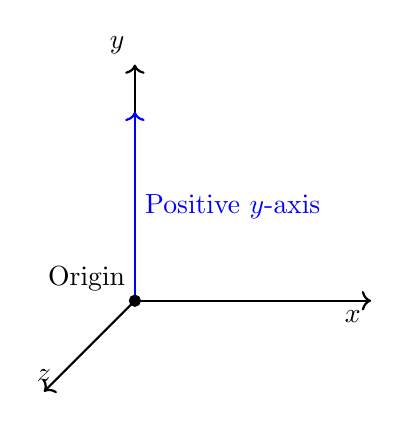
\begin{tikzpicture}[scale=2]

			% Draw the x, y, and z axes
			\draw[->, thick] (0,0,0) -- (1.5,0,0) node[anchor=north east] {$x$};
			\draw[->, thick] (0,0,0) -- (0,1.5,0) node[anchor=south east] {$y$}; % Positive y-axis
			\draw[->, thick] (0,0,0) -- (0,0,1.5) node[anchor=south] {$z$};

			% Positive y-axis with label
			\draw[->, thick, blue] (0,0,0) -- (0,1.2,0) node[midway,right] {Positive $y$-axis};

			% Draw a point at the origin
			\filldraw[black] (0,0,0) circle (1pt) node[anchor=south east] {Origin};

		\end{tikzpicture}
	\end{center}
}

\dfn{Standard Basis Vecotrs}{
	In an $n$-dimensional space $\mathbb{R}^n$, the standard basis vectors are a set of $n$ vectors where each vector has a 1 in one component and 0 in all other components. These vectors are denoted as $\mathbf{e}_i$ for $i = 1, 2, \dots, n$.

	The $i$-th standard basis vector in $\mathbb{R}^n$ is written as:

	\[
		\mathbf{e}_i =
		\begin{pmatrix}
			0                                       \\
			0                                       \\
			\vdots                                  \\
			1 \quad \text{(in the $i$-th position)} \\
			\vdots                                  \\
			0
		\end{pmatrix}
	\]

	For example, in $\mathbb{R}^3$ (three-dimensional space), the standard basis vectors are:

	\[
		\mathbf{e}_1 = \begin{pmatrix} 1 \\ 0 \\ 0 \end{pmatrix}, \quad
		\mathbf{e}_2 = \begin{pmatrix} 0 \\ 1 \\ 0 \end{pmatrix}, \quad
		\mathbf{e}_3 = \begin{pmatrix} 0 \\ 0 \\ 1 \end{pmatrix}.
	\]

	These vectors span the entire vector space $\mathbb{R}^n$, meaning any vector $\mathbf{v} \in \mathbb{R}^n$ can be written as a linear combination of the standard basis vectors:

	\[
		\mathbf{v} = v_1 \mathbf{e}_1 + v_2 \mathbf{e}_2 + \dots + v_n \mathbf{e}_n,
	\]

	where $v_1, v_2, \dots, v_n$ are the components of the vector $\mathbf{v}$.
}

\section{Operations}

\subsection{Dot Product}
\dfn{Dot (Scalar)Product Definitons}{
	The \textbf{scalar product} (or \textbf{dot product}) of two vectors \( \mathbf{a} \) and \( \mathbf{b} \) in \( \mathbb{R}^n \) is defined as:
	\[
		\mathbf{a} \cdot \mathbf{b} = a_1b_1 + a_2b_2 + \dots + a_nb_n
	\]
	In \( \mathbb{R}^3 \), for vectors \( \mathbf{a} = \begin{pmatrix} a_1 \\ a_2 \\ a_3 \end{pmatrix} \) and \( \mathbf{b} = \begin{pmatrix} b_1 \\ b_2 \\ b_3 \end{pmatrix} \), the dot product is:
	\[
		\mathbf{a} \cdot \mathbf{b} = a_1b_1 + a_2b_2 + a_3b_3
	\]
	The dot product can also be expressed in terms of the magnitudes of \( \mathbf{a} \) and \( \mathbf{b} \) and the angle \( \theta \) between them:
	\[
		\mathbf{a} \cdot \mathbf{b} = |\mathbf{a}| |\mathbf{b}| \cos \theta
	\]
	The dot product is a scalar quantity and is zero when the vectors are orthogonal (perpendicular).
	\\
	Useful to find the angle between the two vectors being dot produced together,

}

\thm{Dot Product Proof}{
	We are given the vectors $\vec{v}$ and $\vec{w}$, and we want to express the dot product in terms of their magnitudes and the angle between them.

	Start with the relationship:

	\[
		\vec{x} = \vec{v} - \vec{w}
	\]

	\begin{center}
		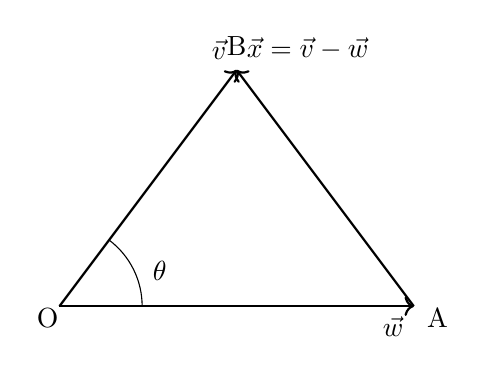
\begin{tikzpicture}[scale=1.5]
			% Draw vectors
			\draw[->, thick] (0,0) -- (3,0) node[anchor=north east] {$\vec{w}$};
			\draw[->, thick] (0,0) -- (1.5,2) node[anchor=south east] {$\vec{v}$};
			\draw[->, thick] (3,0) -- (1.5,2) node[anchor=south west] {$\vec{x} = \vec{v} - \vec{w}$};

			% Label the angle theta
			\draw (0.7,0) arc[start angle=0,end angle=53,radius=0.7];
			\node at (0.85,0.3) {$\theta$};

			% Draw point labels
			\node at (-0.1,-0.1) {O};
			\node at (3.2,-0.1) {A};
			\node at (1.5,2.2) {B};
		\end{tikzpicture}
	\end{center}

	The above diagram illustrates the vectors $\vec{v}$, $\vec{w}$, and their difference $\vec{x} = \vec{v} - \vec{w}$, forming a triangle. The angle $\theta$ is between $\vec{v}$ and $\vec{w}$.

	The magnitude squared of $\vec{x}$ is:

	\[
		|\vec{x}|^2 = |\vec{v}|^2 + |\vec{w}|^2 - 2|\vec{v}||\vec{w}|\cos\theta
	\]

	This is the expansion of the law of cosines.

	Now, from the equation:

	\[
		|\vec{x}|^2 = \sqrt[2]{\left( (v_x - w_x)^2 + (v_y - w_y)^2 \right)}^2
	\]

	We conclude:

	\[
		|\vec{x}|^2 = |\vec{v}|^2 + |\vec{w}|^2 - 2 (\vec{v} \cdot \vec{w})
	\]

	Thus, we can express the dot product $\vec{v} \cdot \vec{w}$ as:

	\[
		\vec{v} \cdot \vec{w} = |\vec{v}||\vec{w}|\cos\theta
	\]
}

\subsection{Applications}

\nt{
	The dot product of two vectors $\vec{v} \cdot \vec{w}$ can take different values, leading to various interpretations of the relationship between the vectors. Below is a table describing some key cases:

	\begin{center}
		\begin{tabular}{|c|c|c|}
			\hline
			\textbf{Dot Product Value}                    & \textbf{Interpretation}         & \textbf{Relationship Between Vectors}                                                         \\
			\hline
			$\vec{v} \cdot \vec{w} = 0$                   & $\cos\theta = 0$                & Vectors are \textbf{perpendicular} (orthogonal), $\theta = 90^\circ$                          \\
			\hline
			$\vec{v} \cdot \vec{w} > 0$                   & $0 < \theta < 90^\circ$         & Vectors form an \textbf{acute angle}, pointing in the same general direction                  \\
			\hline
			$\vec{v} \cdot \vec{w} < 0$                   & $90^\circ < \theta < 180^\circ$ & Vectors form an \textbf{obtuse angle}, pointing in opposite general directions                \\
			\hline
			$\vec{v} \cdot \vec{w} = |\vec{v}||\vec{w}|$  & $\cos\theta = 1$                & Vectors are \textbf{parallel} and point in the \textbf{same direction}, $\theta = 0^\circ$    \\
			\hline
			$\vec{v} \cdot \vec{w} = -|\vec{v}||\vec{w}|$ & $\cos\theta = -1$               & Vectors are \textbf{parallel} but point in \textbf{opposite directions}, $\theta = 180^\circ$ \\
			\hline
		\end{tabular}
	\end{center}
}

\dfn{Vector Product (Cross Product)}{
	The \textbf{vector product} (or \textbf{cross product}) of two vectors \( \mathbf{a} \) and \( \mathbf{b} \) in \( \mathbb{R}^3 \) is a vector \( \mathbf{c} \) that is perpendicular to both \( \mathbf{a} \) and \( \mathbf{b} \), and its magnitude is given by:
	\[
		|\mathbf{c}| = |\mathbf{a} \times \mathbf{b}| = |\mathbf{a}| |\mathbf{b}| \sin \theta
	\]
	where \( \theta \) is the angle between \( \mathbf{a} \) and \( \mathbf{b} \). The cross product is calculated as:
	\[
		\mathbf{a} \times \mathbf{b} = \begin{vmatrix}
			\hat{i} & \hat{j} & \hat{k} \\
			a_1     & a_2     & a_3     \\
			b_1     & b_2     & b_3
		\end{vmatrix} = (a_2b_3 - a_3b_2)\hat{i} - (a_1b_3 - a_3b_1)\hat{j} + (a_1b_2 - a_2b_1)\hat{k}
	\]
	The result of a cross product is a vector perpendicular to the plane formed by \( \mathbf{a} \) and \( \mathbf{b} \), with a direction given by the right-hand rule.
}

\dfn{Vector Projections} {
% Vector projection diagram

\begin{center}
	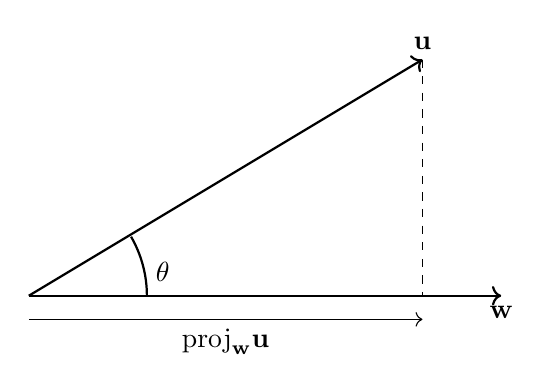
\begin{tikzpicture}
		% Draw vector w
		\draw[->, thick] (0,0) -- (6,0) node[anchor=north] {$\mathbf{w}$};

		% Draw vector u
		\draw[->, thick] (0,0) -- (5,3) node[anchor=south] {$\mathbf{u}$};

		% Projection line
		\draw[dashed] (5,3) -- (5,0) node[anchor=north] {};

		% Angle theta
		\draw[thick] (1.5,0) arc (0:30:1.5);
		\node at (1.7,0.3) {$\theta$};

		% Label projection of u on w
		\draw[->] (0,-0.3) -- (5,-0.3) node[midway,below] {$\text{proj}_{\mathbf{w}}\mathbf{u}$};
	\end{tikzpicture}
\end{center}

\[
	\text{scal}_{\mathbf{w}}\mathbf{u} = |\mathbf{u}| \cdot \cos\theta = \frac{\mathbf{w} \cdot \mathbf{u}}{|\mathbf{w}|}
\]

\[
	\text{proj}_{\mathbf{w}} \mathbf{u} = |\mathbf{u}| \cos \theta \left( \frac{\mathbf{w}}{|\mathbf{w}|} \right)
\]

\[
	\text{proj}_{\mathbf{w}} \mathbf{u} = \left( \frac{\mathbf{w} \cdot \mathbf{u}}{\mathbf{w} \cdot \mathbf{w}} \right) \mathbf{w}
\]
}

\section{Matrix Determinants}

\dfn{Matrix Representation}{
	A matrix is a collection of numbers arranged in a grid format, where each element is positioned based on its row and column. A general $m \times n$ matrix is written as:
	\[
		M =
		\begin{pmatrix}
			a_{11} & a_{12} & \cdots & a_{1n} \\
			a_{21} & a_{22} & \cdots & a_{2n} \\
			\vdots & \vdots & \ddots & \vdots \\
			a_{m1} & a_{m2} & \cdots & a_{mn} \\
		\end{pmatrix}
	\]
	For example, a $2 \times 2$ matrix is given by:
	\[
		M = \begin{pmatrix} a & b \\ c & d \end{pmatrix}
	\]
	A $3 \times 3$ matrix is:
	\[
		M = \begin{pmatrix} a & b & c \\ d & e & f \\ g & h & i \end{pmatrix}
	\]
	Matrices can be considered as a collection of vectors where each row or column can represent a vector.
}

\nt{\textbf{Vector Representation} \\
	A matrix can also be viewed as a collection of vectors. For instance, a $3 \times 3$ matrix can be interpreted as:
	\[
		M = \begin{pmatrix}
			\vec{v_1} = \langle a, b, c \rangle \\
			\vec{v_2} = \langle d, e, f \rangle \\
			\vec{v_3} = \langle g, h, i \rangle
		\end{pmatrix}
	\]
	where each row (or column) is treated as a vector in space.
}

\dfn{Determinant of a $2 \times 2$ Matrix}{
	The determinant of a $2 \times 2$ matrix is given by:
	\[
		\text{det}(M) = \det\begin{pmatrix} a & b \\ c & d \end{pmatrix} = ad - bc
	\]
	The determinant represents the signed area of the parallelogram formed by the vectors corresponding to the rows (or columns) of the matrix.


	\begin{center}
		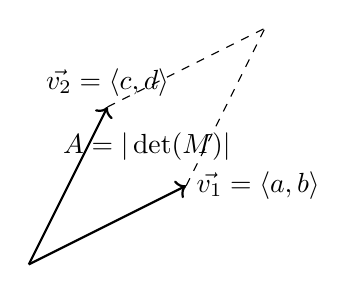
\begin{tikzpicture}
			% Define the vectors
			\draw[->, thick] (0,0) -- (2,1) node[right] {$\vec{v_1} = \langle a, b \rangle$};
			\draw[->, thick] (0,0) -- (1,2) node[above] {$\vec{v_2} = \langle c, d \rangle$};

			% Draw the parallelogram
			\draw[dashed] (2,1) -- (3,3);
			\draw[dashed] (1,2) -- (3,3);

			% Label the area
			\node at (1.5, 1.5) {$A = |\det(M)|$};
		\end{tikzpicture}
	\end{center}

}

\nt{\textbf{Geometric Interpretation} \\
	For a $2 \times 2$ matrix, the determinant represents the area $A$ of the parallelogram formed by the two vectors $\vec{v_1} = \langle a, b \rangle$ and $\vec{v_2} = \langle c, d \rangle$. The magnitude of the determinant gives the area of this parallelogram, and the sign of the determinant indicates the orientation (whether the vectors are ordered clockwise or counterclockwise).
}

\dfn{Determinant of a $3 \times 3$ Matrix}{
	The determinant of a $3 \times 3$ matrix is calculated as:
	\[
		\text{det}(M) = \det \begin{pmatrix}
			a & b & c \\
			d & e & f \\
			g & h & i
		\end{pmatrix}
		= a \det \begin{pmatrix} e & f \\ h & i \end{pmatrix}
		- b \det \begin{pmatrix} d & f \\ g & i \end{pmatrix}
		+ c \det \begin{pmatrix} d & e \\ g & h \end{pmatrix}
	\]
	The determinant represents the signed volume of the parallelepiped formed by the three vectors corresponding to the rows (or columns) of the matrix.
	\begin{center}
		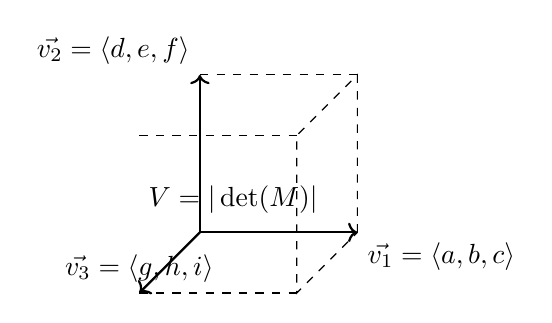
\begin{tikzpicture}
			% Define the 3D vectors
			\draw[->, thick] (0,0,0) -- (2,0,0) node[below right] {$\vec{v_1} = \langle a, b, c \rangle$};
			\draw[->, thick] (0,0,0) -- (0,2,0) node[above left] {$\vec{v_2} = \langle d, e, f \rangle$};
			\draw[->, thick] (0,0,0) -- (0,0,2) node[above] {$\vec{v_3} = \langle g, h, i \rangle$};

			% Draw the parallelepiped
			\draw[dashed] (2,0,0) -- (2,2,0) -- (2,2,2) -- (2,0,2) -- cycle;
			\draw[dashed] (0,2,0) -- (2,2,0);
			\draw[dashed] (0,0,2) -- (2,0,2);
			\draw[dashed] (0,2,2) -- (2,2,2);

			% Label the volume
			\node at (1,1,1.5) {$V = |\det(M)|$};
		\end{tikzpicture}
	\end{center}

}

\nt{\textbf{Geometric Interpretation for $3 \times 3$} \\
	In the $3 \times 3$ case, the determinant represents the volume $V$ of the parallelepiped formed by three vectors $\vec{v_1}, \vec{v_2}, \vec{v_3}$, and the sign indicates whether the orientation is right-handed or left-handed. The magnitude gives the volume.
}

\section{Matrix multiplication with 2D Vectors}

\dfn{Vector Matrix Multiplication}{

	\[
		M = \begin{pmatrix} a_{11} & a_{12} \\ a_{21} & a_{22} \end{pmatrix}, \quad
		V = \begin{pmatrix} V_1 \\ V_2 \end{pmatrix}
	\]

	\[
		\hat{\mathbf{j}}M = \langle a_{11}V_1 + a_{12}V_2, a_{21}V_1 + a_{22}V_2 \rangle
	\]

	Given:
	\[
		\hat{i} = \langle 1, 0 \rangle \quad \hat{j} = \langle 0, 1 \rangle
	\]

	We can compute:
	\[
		iM = \langle a_{11}, a_{12} \rangle = a_1
	\]
	\[
		jM = \langle a_{21}, a_{22} \rangle = a_2
	\]

	Where:
	\[
		\mathbf{V} = V_1 \hat{i} + V_2 \hat{j}
	\]
	\[
		\hat{\mathbf{V}}M = \left( V_1 \hat{i} + V_2 \hat{j} \right) M
	\]
	\[
		= V_1 \hat{i} M + V_2 \hat{j} M
	\]
	\[
		= V_1 \mathbf{a}_1 + V_2 \mathbf{a}_2
	\]

}

\nt{
	\centering
	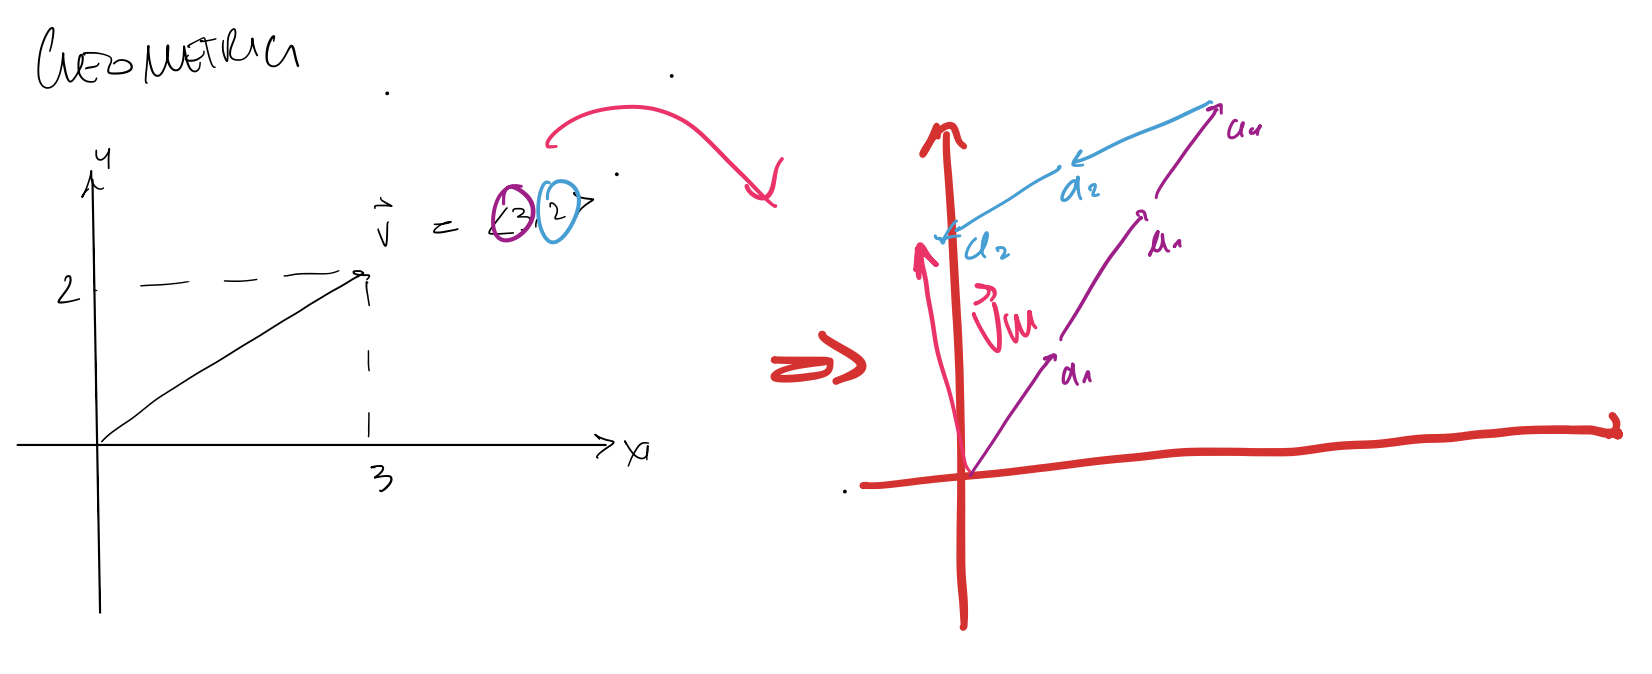
\includegraphics[width=0.5\textwidth]{graphicalvm.png} % Adjust the width as needed
	\par\vspace{1em} % Adds a small space after the image
}

\subsection{Effect on Area}

\dfn{$2D$}{
The original point \( (1,1) \) is transformed by the matrix \( M \). This transformation impacts the area and orientation as follows:

\[
	M = \begin{pmatrix} a_{11} & a_{12} \\ a_{21} & a_{22} \end{pmatrix}
\]

The area after transformation is given by the determinant of the matrix:

\[
	\text{Area} = \det(M)
\]
Where the determinant is calculated as:
\[
	\det(M) = a_{11}a_{22} - a_{12}a_{21}
\]

The determinant also determines the orientation:
\[
	\det(M) = \begin{cases}
		A  & \text{if } a_1 \text{ to } a_2 \text{ is counterclockwise} \\
		-A & \text{otherwise}
	\end{cases}
\]

In the example, the original vectors \( a_1 \) and \( a_2 \) form an area, and the determinant will tell us if the vectors are oriented in a clockwise or counterclockwise fashion.

If the determinant is negative, the orientation is clockwise, as illustrated:

\[
	\det \left( \begin{pmatrix} a_1 & a_2 \end{pmatrix} \right) < 0
\]

Thus, in this case, the transformation results in a clockwise orientation.
}

\section{Matrix multiplication with 3D Vectors}

\dfn{$3D$}{
	The matrix \( M \) for a 3D transformation is given as:

	\[
		M = \begin{pmatrix}
			a_{11} & a_{12} & a_{13} \\
			a_{21} & a_{22} & a_{23} \\
			a_{31} & a_{32} & a_{33}
		\end{pmatrix}
		\quad
		\text{where} \quad
		\vec{V} = \langle V_1, V_2, V_3 \rangle
	\]

	The transformation of vector \( \vec{V} \) under matrix \( M \) is:

	\[
		\hat{\vec{V}} M = \langle (a_{11} V_1 + a_{12} V_2 + a_{13} V_3), (a_{21} V_1 + a_{22} V_2 + a_{23} V_3), (a_{31} V_1 + a_{32} V_2 + a_{33} V_3) \rangle
	\]

	This can be written in terms of the basis vectors as:
	\[
		\left( V_1 \hat{i} + V_2 \hat{j} + V_3 \hat{k} \right) M = V_1 \vec{a}_1 + V_2 \vec{a}_2 + V_3 \vec{a}_3
	\]

}

\dfn{orientation and Volume}{
- If the determinant of matrix \( M \) is negative, the system is **left-handed**, i.e.,
\[
	\det(M) = -V
\]
- The determinant of the matrix \( M \) gives the **volume** of the parallelepiped spanned by the vectors \( a_1, a_2, a_3 \):

\[
	\det(M) = \text{Volume}(V)
\]

The volume \( V \) is given by:
\[
	V = \begin{cases}
		+V & \text{if } \vec{a}_1, \vec{a}_2, \vec{a}_3 \text{ are right-handed (RHS)} \\
		-V & \text{otherwise (left-handed)}
	\end{cases}
\]
}

\section{Cross Product and Volumes}

\dfn{Cross Product and Volumes}{
	The volume of a parallelepiped defined by three vectors \( \vec{u}, \vec{v}, \vec{w} \) is given by:
	\[
		\text{V} = \vec{u} \cdot (\vec{v} \times \vec{w})
	\]
}

\subsection{Link to Matrix Determinants}

\dfn{Cross Product and Matrix Determinants}{
	\textbf{Since:}
	\[
		\vec{u} \cdot (\vec{v} \times \vec{w}) = \det \begin{pmatrix} \vec{u} & \vec{v} & \vec{w} \end{pmatrix}
	\]

	\[
		\det \begin{pmatrix}
			u_1 & u_2 & u_3 \\
			v_1 & v_2 & v_3 \\
			w_1 & w_2 & w_3
		\end{pmatrix}
		=
		u_1 \det \begin{pmatrix} v_2 & v_3 \\ w_2 & w_3 \end{pmatrix}
		- u_2 \det \begin{pmatrix} v_1 & v_3 \\ w_1 & w_3 \end{pmatrix}
		+ u_3 \det \begin{pmatrix} v_1 & v_2 \\ w_1 & w_2 \end{pmatrix}
	\]

	\[
		= \vec{u} \cdot
		\left(
		\hat{i} \begin{vmatrix} v_2 & v_3 \\ w_2 & w_3 \end{vmatrix}
		- \hat{j} \begin{vmatrix} v_1 & v_3 \\ w_1 & w_3 \end{vmatrix}
		+ \hat{k} \begin{vmatrix} v_1 & v_2 \\ w_1 & w_2 \end{vmatrix}
		\right)
	\]

	\[
		= \vec{u} \cdot \det \begin{pmatrix} \hat{i} & \hat{j} & \hat{k} \\ v_1 & v_2 & v_3 \\ w_1 & w_2 & w_3 \end{pmatrix}
	\]

	\[
		= \vec{u} \cdot (\vec{v} \times \vec{w})
	\]

	\textbf{Therefore:}

	\[
		\vec{v} \times \vec{w} = \det \begin{pmatrix} \hat{i} & \hat{j} & \hat{k} \\ v_1 & v_2 & v_3 \\ w_1 & w_2 & w_3 \end{pmatrix}
	\]
}

\section {Cross Product Polynomial Multiplication}

\dfn{Properties}{

	\[
		\hat{i} \times \hat{j} = \hat{k}, \quad \hat{j} \times \hat{k} = \hat{i}, \quad \hat{k} \times \hat{i} = \hat{j}
	\]

	\[
		\hat{j} \times \hat{i} = -\hat{k}, \quad \hat{i} \times \hat{i} = \hat{j} \times \hat{j} = \hat{k} \times \hat{k} = 0
	\]
}

\ex{Example: Cross Product}{
	Let \( \vec{v} = 2\hat{i} - \hat{j} - 3\hat{k} \) and \( \vec{w} = \hat{i} + \hat{j} + \hat{k} \). The cross product \( \vec{v} \times \vec{w} \) is computed as:

	\[
		\vec{v} \times \vec{w} = \left( 2\hat{i} - \hat{j} - 3\hat{k} \right) \times \left( \hat{i} + \hat{j} + \hat{k} \right)
	\]

	Expanding the cross product term by term:

	\[
		= 2\hat{i} \times \hat{i} + 2\hat{i} \times \hat{j} + 2\hat{i} \times \hat{k}
		- \hat{j} \times \hat{i} - \hat{j} \times \hat{j} - \hat{j} \times \hat{k}
		- 3\hat{k} \times \hat{i} - 3\hat{k} \times \hat{j} - 3\hat{k} \times \hat{k}
	\]

	Using the cross product identities:

	\[
		= 0 + 2\hat{k} + 2(-\hat{j})
		- (-\hat{k}) + 0 - \hat{i}
		- 3\hat{j} + 3\hat{i} + 0
	\]

	Combining like terms:

	\[
		= (3\hat{i} - \hat{i}) + (-2\hat{j} - 3\hat{j}) + (2\hat{k} + \hat{k})
	\]

	\[
		= 2\hat{i} - 5\hat{j} + 3\hat{k}
	\]

	Thus, the final result is:

	\[
		\vec{v} \times \vec{w} = 2\hat{i} - 5\hat{j} + 3\hat{k}
	\]
}

\end{document}